% Generated by tex/build_swebok_structure.py from tex/chapters/ch01/03_ソフトウェア要求の基礎.tex
\subsubsection{ソフトウェア要求活動}

要求活動は、大きく\term{要求開発}と\term{要求管理}に分けられる。

\term{要求開発}は、「何を作るか」について合意を作る活動である。具体的には、\term{要求獲得}、\term{要求分析}、\term{要求仕様化}、\term{要求妥当性確認}を含む。

\term{要求管理}は、その合意を時間とともに維持する活動である。要求は開発中にも保守中にも変化するため、不要な要求の整理、変更要求の扱い、スコープと予算・納期の調整が必要になる。

\begin{figure}[htbp]
\centering
\IfFileExists{swebok_structure/CH01.ソフトウェア要求(Software_Requirements)/1.1.ソフトウェア要求の基礎(Software_Requirements_Fundamentals)/1.1.11.ソフトウェア要求活動(Software_Requirements_Activities)/assets/fig-ch01-05.png}{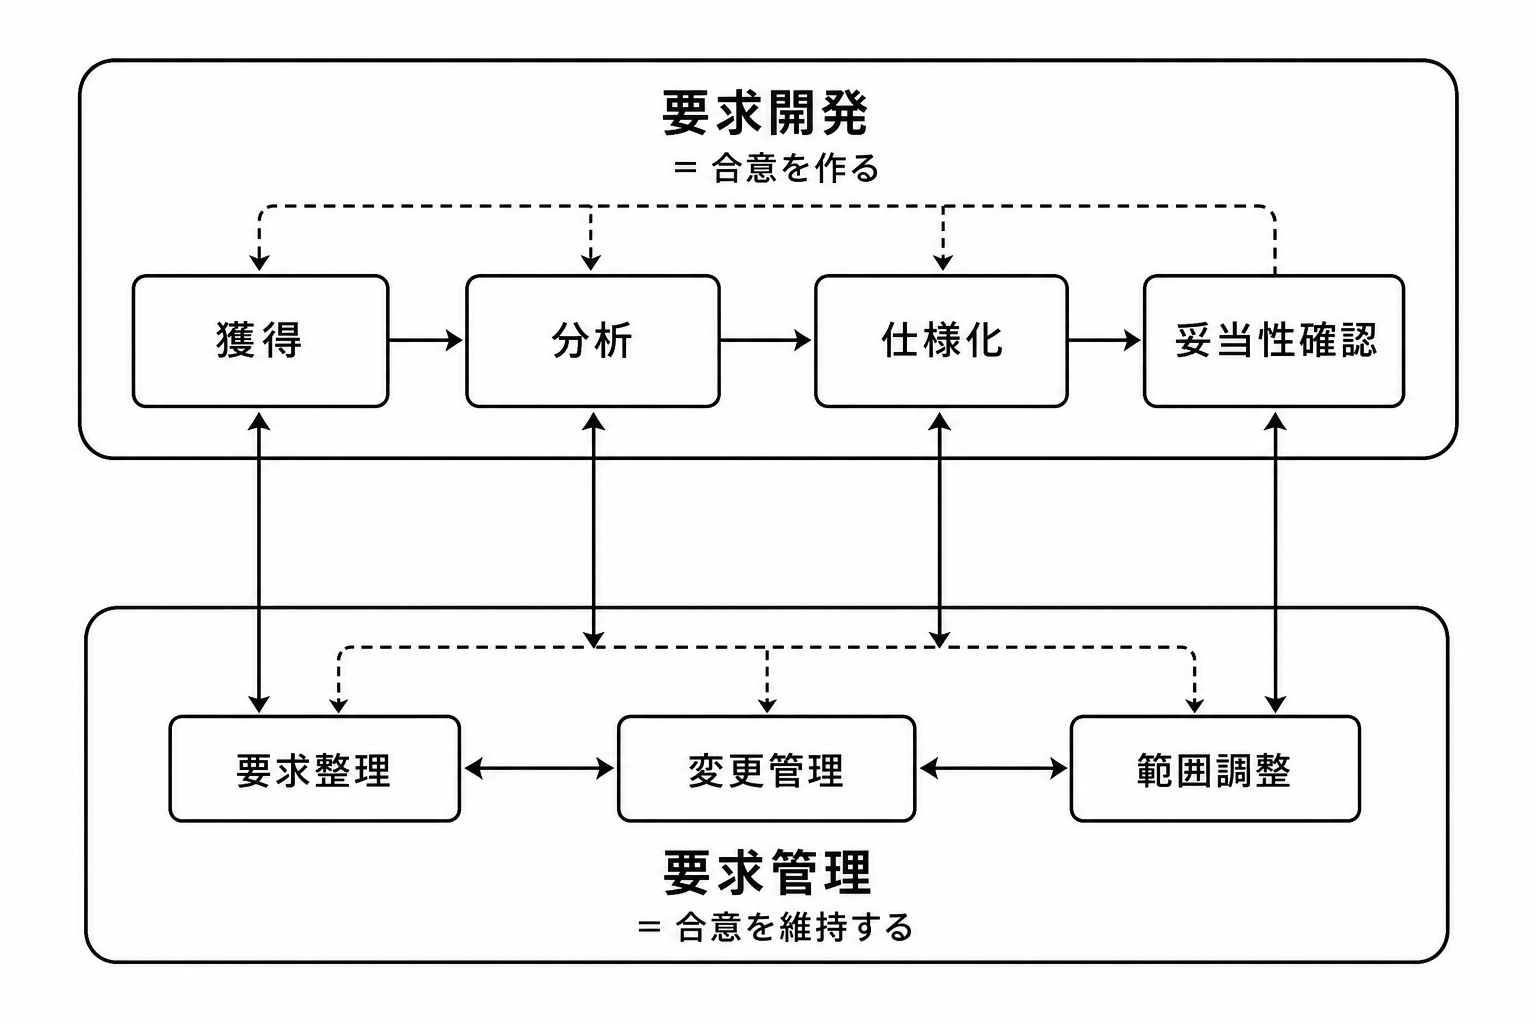
\includegraphics[width=0.96\linewidth]{swebok_structure/CH01.ソフトウェア要求(Software_Requirements)/1.1.ソフトウェア要求の基礎(Software_Requirements_Fundamentals)/1.1.11.ソフトウェア要求活動(Software_Requirements_Activities)/assets/fig-ch01-05.png}}{\fbox{\parbox[c][48mm][c]{0.9\linewidth}{\centering 画像生成待ち\\要求開発と要求管理の活動図}}}
\caption{要求開発と要求管理の活動図}
\label{fig:ch01-05}
\end{figure}
